


























































\subsection{Dark Matter Particle Physics}
\label{sec:dm_particle_physics}

% this paragraph should be shortened. It should state what dark matter is and then state the problem of the discrepancy of clear presence in astronomy but missing in particle physics and state that it is therefore one of the largest problems in physics. The next paragraph should merely give the reader an overview of the subsections in dark matter particle physics.

%\gls{dm} is an invisible and hypothetical form of matter motivated by astronomical studies that imply that \gls{dm} has a gravitational interaction with normal matter, i.e the matter that is included in the \gls{sm} of particle physics. Yet there are no experiments that have been able to detect \textit{\gls{dm} particles}, prove the creation of \gls{dm}, or prove a theory that explains \gls{dm} at the subatomic level. In cosmology \gls{dm} is a widely accepted explanation for observed gravitational effects of celestial bodies that cannot solely be explained by general relativity and normal matter. The bridge of \gls{dm} in cosmology to particle physics has not been trivial. By modern standards, however, this pressing discrepancy between \gls{dm}'s clear presence in cosmology and \gls{dm}'s absence in particle physics is perhaps the largest reason for why it is considered one of the largest unsolved problems in modern physics. \cite{bertone2016-history-dark-matter} \cite{cirelli2026-darkmatter} 

\Gls{dm} is the name given to a proposed form of invisible matter that does not
emit, absorb or scatter light. Astronomical and cosmological measurements reveal
gravitational effects that, within general relativity, cannot be explained by the
observed distribution of ordinary matter alone. Dark matter is the leading
explanation for these observations, but their cause has not been directly
established. In particular, no \gls{dm} particle or non-gravitational interaction
with the particles of the \gls{sm} has been confirmed in an experiment. This gap
between well-established astronomical observations and an unknown subatomic
explanation makes dark matter one of the largest unsolved problems in modern
physics \cite{bertone2016-history-dark-matter,cirelli2026-darkmatter}.


%\gls{dm} is the name given to an invisible matter that does not emit, absorb or scatter light, but whose gravitational influence is observed throughout the Universe.  Astronomical and cosmological measurements provide strong evidence %This line should not imply that it provides strong evidence for it, but rather dark matter is an explanation to explain observations of gravitational effects that cannot be referenced to normal matter for its presence,  yet no \gls{dm} particle or non-gravitational interaction with the particles of the \gls{sm} has been confirmed in an experiment. This gap between clear astronomical evidence and an unknown subatomic explanation makes dark matter one of the largest unsolved problems in modern physics \cite{bertone2016-history-dark-matter,cirelli2026-darkmatter}.



% UPDATE
%This subsection will give the reader a brief historical context to \gls{dm} and its introduction in particle physics, an introduction to the thermal freeze out framework that gives thermal relic \gls{dm}, and lastly a description of the Dark Bremsstrahlung particle interaction that is the basis for the \gls{ldmx}.

This subsection briefly traces the introduction of \gls{dm} into particle
physics before presenting thermal freeze-out, light dark matter and the dark
bremsstrahlung process that is the basis for the \gls{ldmx}.

\subsubsection{A Brief History of Dark Matter: from Astronomy to Particle Physics}
\label{sec:history}

%At the frontier of observation, a new tool can change what is visible. When Galileo Galilei (17th century) pointed the telescope at the sky, he measured that the movement of Jupiter had irregularities, implying 4 satellites of mass orbiting it, but the moons were invisible to the naked eye. These were not discoveries of \gls{dm}, but they illustrate two important ideas: nature may contain matter beyond the reach of ordinary perception, and a new instrument can move that reach \cite{bertone2016-history-dark-matter}. Just as the telescope did not create Galileo's moons, a reconstruction algorithm does not create new detector information either, it attempts to make better use of information that is already there.

At the frontier of observation, a new tool can change what is visible. When
Galileo Galilei pointed his telescope at the sky in the 17th century, he
resolved the faint glow of the Milky Way into stars and observed four
satellites in orbit around Jupiter, all previously invisible to the naked eye.
These were not discoveries of \gls{dm}, but they illustrate two important ideas:
nature may contain matter beyond the reach of ordinary perception, and a new
instrument can move that reach \cite{bertone2016-history-dark-matter}. Just as
the telescope did not create Galileo's moons, a reconstruction algorithm does
not create new detector information either, it attempts to make better use of
information that is already there.



\gls{dm} as a concept encapsulates this idea of matter that exists, but cannot
be perceived by ordinary means. The history of the physical phenomenon now
called dark matter, however, begins with measurements that revealed more
gravitating mass than astronomers could see. Astronomers could estimate the
visible mass of a galaxy or galaxy cluster from its light and independently
estimate the total mass required to explain how its stars or galaxies moved.
Several studies independently found that the visible mass was not enough. 
These studies included the recently rediscovered work by Lund University astronomer Knut Lundmark, whose
1930 comparison of the luminosities and mass estimates of five galaxies
preceded Fritz Zwicky's more famous 1933 study of the Coma cluster. Zwicky borrowed
the virial theorem from thermodynamics, modeling celestial bodies as particles, to show that the galaxies in Coma moved too rapidly for the
cluster to be held together by its visible mass alone.
Later measurements of galactic rotation curves showed a related
discrepancy: stars far from galactic centres moved faster than expected from the
visible matter
\cite{lundmark1930-galaxy-masses,bertone2016-history-dark-matter,
orodruin2016-lundmark-darkmatter}. For these astronomers, however, ``dark
matter'' generally meant unseen astronomical material such as faint stars, cold
gas or other non-luminous bodies, not necessarily a new elementary particle.

The transition from unseen astronomical matter to particle physics was neither
immediate nor automatic. It required both new evidence and a change in
scientific culture. Half a century ago, cosmology was still regarded by many physicists as a ''fringe science'' with limited predictive
power and testability, and the two communities rarely contributed to each
other's fields \cite{bertone2016-history-dark-matter}.

As cosmology became a recognized quantitative science, measurements of primordial element
abundances and the cosmic microwave background showed that baryonic
matter could not provide all the required mass. Within the standard
cosmological model, baryonic matter, meaning ordinary matter composed primarily
of protons and neutrons, accounts for only about \(16\%\) of the total matter
in the Universe. The remaining \(84\%\) is attributed to dark matter
\cite{cirelli2026-darkmatter}. Studies of structure formation further indicate
that the dominant component must have moved slowly enough to behave as cold matter. These results helped transform dark matter from a problem of unseen
astronomical objects into a problem that could require new particle physics.

Modified-gravity explanations, which attempt to reproduce these observations
without introducing a new non-baryonic matter component, have also been
explored, but none has accounted for the full range of observations as
successfully as the dark matter framework
\cite{bertone2016-history-dark-matter,cirelli2026-darkmatter}. 
%Even so, the astronomical observations are still isolated to a phenomenon of gravity and they do not by themselves establish that its cause is a particle.

The \gls{sm} describes the known elementary particles and their strong, weak
and electromagnetic interactions, while gravity is disconnected described separately by
general relativity. No known \gls{sm} particle simultaneously has the
properties required to account for the observed cold dark matter. A particle
interpretation therefore points beyond the \gls{sm}, to possibly a \gls{dm} sector. 
%A particle interpretation of dark matter therefore requires physics beyond the \gls{sm}. 
A viable \gls{dm} particle
candidate must have three key properties:




% I have made this enumerate exactly how I want it I needed to make it easier to read. 
\begin{enumerate}
    \item \textbf{Mass.} A \gls{dm} particle candidate must have mass higher than zero, accounting for the invisible mass in the Universe, and it explains its gravitational influence.
    \item \textbf{Stability.} 
    Observations in the cosmic microwave background imply 
    the existence of \gls{dm} in the early Universe and it remains abundant today. It must therefore be stable, or at least have a lifetime long
    enough to survive until the present day.
    \item \textbf{Almost no interaction with the \gls{sm}.} Gravity is described separately from the \gls{sm}, but it is the only established interaction between \gls{dm} and ordinary matter. \textbf{\emph{If}} \gls{dm} has any additional interactions with \gls{sm} particles, they must be sufficiently weak to have escaped detection in previous experiments. In particular, any electromagnetic interaction must be extremely weak.
\end{enumerate}


\subsubsection{Thermal Relics and the Sub-GeV Frontier}
\label{sec:thermal_relic}


Possible dark matter candidates span an enormous range of masses.
Figure~\ref{fig:dm_candidate_range} gives a schematic overview of several
frequently discussed regions. In this thesis, \gls{ldm} refers to particle dark
matter below approximately the GeV mass scale. The range of greatest relevance to
\gls{ldmx} is roughly from MeV to GeV masses. 
%\gls{ldm} is not one specific particle model, it is a lower-mass region containing many possible candidates and interaction mechanisms
\cite{battaglieri2017-cosmic-visions,ldmx2025-overview}.

\begin{figure}[htbp]
    \centering
    
\includegraphics[width=\linewidth]{config/fig/dm_range.jpeg}
    \caption{Representative mass ranges for several \gls{dm} candidates and frameworks. The \gls{ldm} region relevant to LDMX is highlighted in magenta, while WIMP benchmarks occupy a higher-mass part of the broader thermal dark matter region. The boundaries are illustrative and model-dependent. Reproduced from Figure~4 of Ref.~\cite{gajdan2025-hcal-thesis}, which was inspired by Figure~1 of Ref.~\cite{battaglieri2017-cosmic-visions}.}
    \label{fig:dm_candidate_range}
\end{figure}

The \emph{thermal freeze-out} hypothesis is one possible explanation for the
amount of dark matter observed today. In this model one assumes that there exists an interaction
that connects the \gls{sm} and the dark sector. Given this assumption, in the hot and dense early Universe, particle collisions were frequent and energetic enough to create dark matter particles. Dark matter particles could also annihilate back into \gls{sm} particles. These reactions occurred rapidly enough to keep the two
sectors in \emph{thermal equilibrium}. 


As the Universe expanded, it became cooler and less dense. Creating massive
dark matter particles became increasingly difficult, while existing dark matter
particles continued to annihilate. Eventually, the particles became so dilute
that the annihilation rate fell below the expansion rate of the Universe.
Annihilation then became rare, and the number of dark matter particles in a
volume expanding with the Universe remained approximately constant. Their abundance had \emph{frozen out}, and the surviving population is called
a \emph{thermal relic}.

The surviving thermal relic depends on the strength of the interaction. A stronger
annihilation process remains effective for longer and leaves fewer dark matter
particles, while a weaker process causes an earlier freeze-out and leaves more
particles. For a specified particle model and mass, the observed dark matter
abundance therefore defines a target interaction strength
\cite{cirelli2026-darkmatter}. This is referred to as the \emph{thermal target}.
Thermal freeze-out does not define one universal dark matter mass range because
the result also depends on the particle model, its interactions and the history
of the early Universe.

The historically best-known thermal relic candidate is the \gls{wimp}. A
particle with a mass near the electroweak scale with a weak-strength interaction can freeze
out with approximately the observed abundance, a coincidence known as the
\emph{WIMP miracle}. Searches have strongly constrained many WIMP models
without finding a confirmed signal, although WIMPs as a class have not been
excluded. Experimental limits depend on both particle mass and interaction
strength. Below the GeV scale, the nuclear recoil produced by a dark matter
particle becomes difficult for traditional WIMP searches to detect, motivating
alternative searches for \gls{ldm}
\cite{cirelli2026-darkmatter,krnjaic2026-thermal-dark-photon,
ldmx2025-overview}.



\begin{figure}[htbp]
    \begin{minipage}[t]{0.48\linewidth}
        \centering
        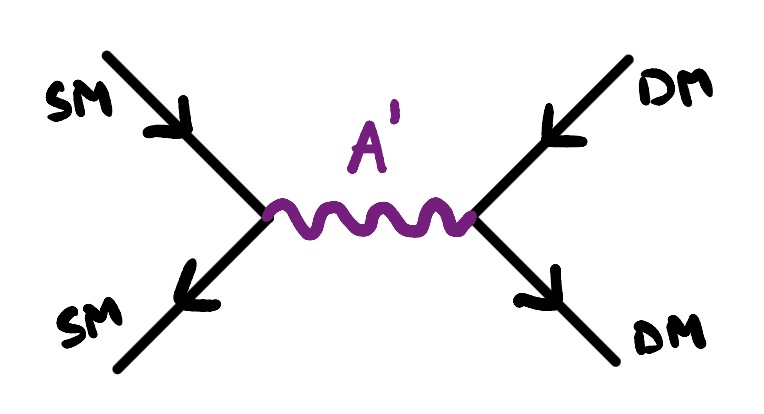
\includegraphics[width=\linewidth]{config/fig/dark_photon_feynman.jpg}
        \caption{Feynman diagram of conversion of a pair of \gls{sm} particles into a
        pair of \gls{dm} particles, mediated by a dark photon \(A'\).}
        \label{fig:sm_dm_dark_photon}
    \end{minipage}
    \hfill
    \begin{minipage}[t]{0.48\linewidth}
        \centering
        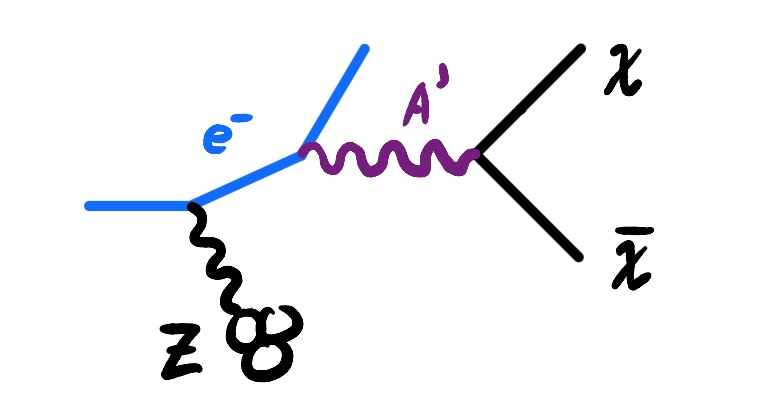
\includegraphics[width=\linewidth]{config/fig/dark_bremsstrahlung_feynman.jpg}
        \caption{Feynman diagram-sketch of dark bremsstrahlung.
        %in electron-nucleus scattering.
        The electron scatters and radiates a dark photon \(A'\), which decays into
        an invisible dark matter particle-antiparticle pair \(\chi\bar{\chi}\). The
        recoiling electron provides a visible signature by the law of conservation of momentum. Inspired by Ref.~\cite{helgstrand2025veto_power}.}
        \label{fig:dark_bremsstrahlung_feynman}
    \end{minipage}
\end{figure}

One way to connect \gls{ldm} to the \gls{sm} introduces
a new dark-sector gauge-boson mediator called the \gls{dark photon}, denoted by \(A'\) in
Figure~\ref{fig:sm_dm_dark_photon}. It can be
thought of as a dark-sector relative of the ordinary photon. A small kinetic mixing with the ordinary
photon allows the dark photon to interact weakly with electrically charged
\gls{sm} particles. In the invisible dark photon benchmark considered here, the dark
photon decays into a pair of dark matter particles, denoted by
\(\chi\bar{\chi}\)
\cite{cirelli2026-darkmatter,ldmx2025-overview}.


%An incoming electron scatters in the field of a target nucleus and radiates a dark photon, which decays into \(\chi\bar{\chi}\). The dark matter particles leave no measurable detector signal, but their production can instead be inferred from the imbalance between the incoming electron momentum and the reconstructed visible final state.


In an electron fixed-target experiment, the benchmark production reaction is
\emph{dark bremsstrahlung}, illustrated in
Figure~\ref{fig:dark_bremsstrahlung_feynman}. It is a dark-sector version of
ordinary bremsstrahlung. An incoming electron scatters in the field of a target
nucleus and radiates a dark photon, which then decays into
\(\chi\bar{\chi}\). The dark matter particles leave no measurable detector
signal. Their production can instead be inferred from the imbalance between
the incoming electron momentum and the reconstructed visible final state.
Unexplored thermal targets motivate the missing-momentum search for which
\gls{ldmx} is designed
\cite{akesson2018-ldmx,ldmx2025-overview}.

Dark bremsstrahlung turns the original astronomical question into a tangible
experimental one: can missing momentum reveal an invisible final state after
ordinary sources of imbalance have been rejected? The next subsection
introduces the detector built to answer that question.





\subsection{The Light Dark Matter eXperiment}
\label{sec:ldmx}

\subsubsection{Search Strategy and Physics Goal}
% This section is good in what it achieves and what it wants to tell, but the parts preceding this has been rewritten since and now there is dual information this section does not have to explain stuff again that was explained in previous section. An overview and review of this part with previous parts in mind is necessary. 

% I think this section is missing the perspective of what researches and collaborators are involved in this. It is cool to mention in one sentence in the first paragraph that it is planned in california the us but collaborators are also in other places of the world. 

% I think it would be suitable to explain the choice of tungsten, why tungsten materials? Bremsstrahluhn is implied to be relevant and to occur with tungsten, that could be explicitly stated in 1 sentence with very short explanation.

%Dark bremsstrahlung provides the main benchmark production process for the \gls{ldmx}. LDMX is an electron fixed-target \gls{missing momentum experiment} designed to search for sub-GeV \gls{dm}. An \(8\,\mathrm{GeV}\) electron beam will strike a thin tungsten target at End Station A at \gls{slac}. The momentum of each incoming electron is compared with the measured momentum and energy in the final state. A large imbalance can indicate that an invisible particle carried momentum out of the detector \cite{ldmx2025-overview}.

\Gls{ldmx} is an electron fixed-target \textit{missing momentum} experiment
designed to search for sub-GeV \gls{dm} through the dark-bremsstrahlung
process introduced above. The experiment is planned for End Station A at
\gls{slac} outside of San Francisco, California and is developed by an international collaboration
with institutions in the United States and Sweden. An \(8\,\mathrm{GeV}\)
electron beam will strike a thin tungsten target. Tungsten is used because
its high atomic number gives a large production rate for low-mass dark
photons and helps reduce nuclear backgrounds at the chosen target thickness
\cite{ldmx2025-overview}.






% The explanations here have been repeated from the previous dark matter chapter. We should not repeat stuff find a way new formulation that goes straight to the point instead and trusts that the reader has read the previous part or can just simply do so if one wants to. 
In the dark bremsstrahlung benchmark, the beam electron radiates a
\gls{dark photon}, denoted \(A'\). The mediator couples weakly to electrically
charged \gls{sm} particles and can decay into a pair of dark-sector particles,
denoted by \(\chi\). It therefore provides a possible bridge between the
\gls{sm} and a dark sector. The \gls{dm} particles do not produce a
measurable detector signal. LDMX instead tests the model by searching for the
recoil of the electron and the missing momentum left by their production
\cite{akesson2018-ldmx,ldmx2025-overview}.

In the benchmark process, a candidate event has three main features. The electron leaves the target
with less energy than it entered with, it receives a transverse (perpendicular to the beam direction)
momentum kick, and no other visible final-state particle accounts for the
lost momentum. The combination is important because ordinary
\gls{sm} interactions can mimic parts of this signature when a
visible particle escapes detection. The trackers therefore measure the
incoming and recoil-electron momenta, while the calorimeters test whether
additional visible activity explains the apparent missing momentum
\cite{akesson2018-ldmx,ldmx2025-overview}.

The planned beam structure delivers approximately 20 million filled buckets
per second, with an average of one to two electrons in each bucket. This
corresponds to roughly 20 to 40 million electrons reaching the target per
second during operation. The exposure, measured in \gls{eot}, is not a
universal event count required to reject a null hypothesis. Rather, increasing
the exposure increases sensitivity to rarer production processes and weaker
interactions. The attainable exposure also depends on running time, detector
performance, backgrounds and radiation tolerance. LDMX is designed for a
staged programme beginning around \(4\times10^{14}\) \gls{eot} and extending
towards exposures of order \(10^{16}\) \gls{eot}, with projected sensitivity
up to three orders of magnitude beyond earlier searches
\cite{ldmx2025-overview}.

Useful exposure depends not only on how many electrons are delivered, but
also on which events can be triggered, stored and reconstructed. The ability
to retain events containing several electrons can therefore improve the
practical physics reach. This connection is developed further in
Section~\ref{sec:formalism}.

\begin{figure}[H]
    \centering
    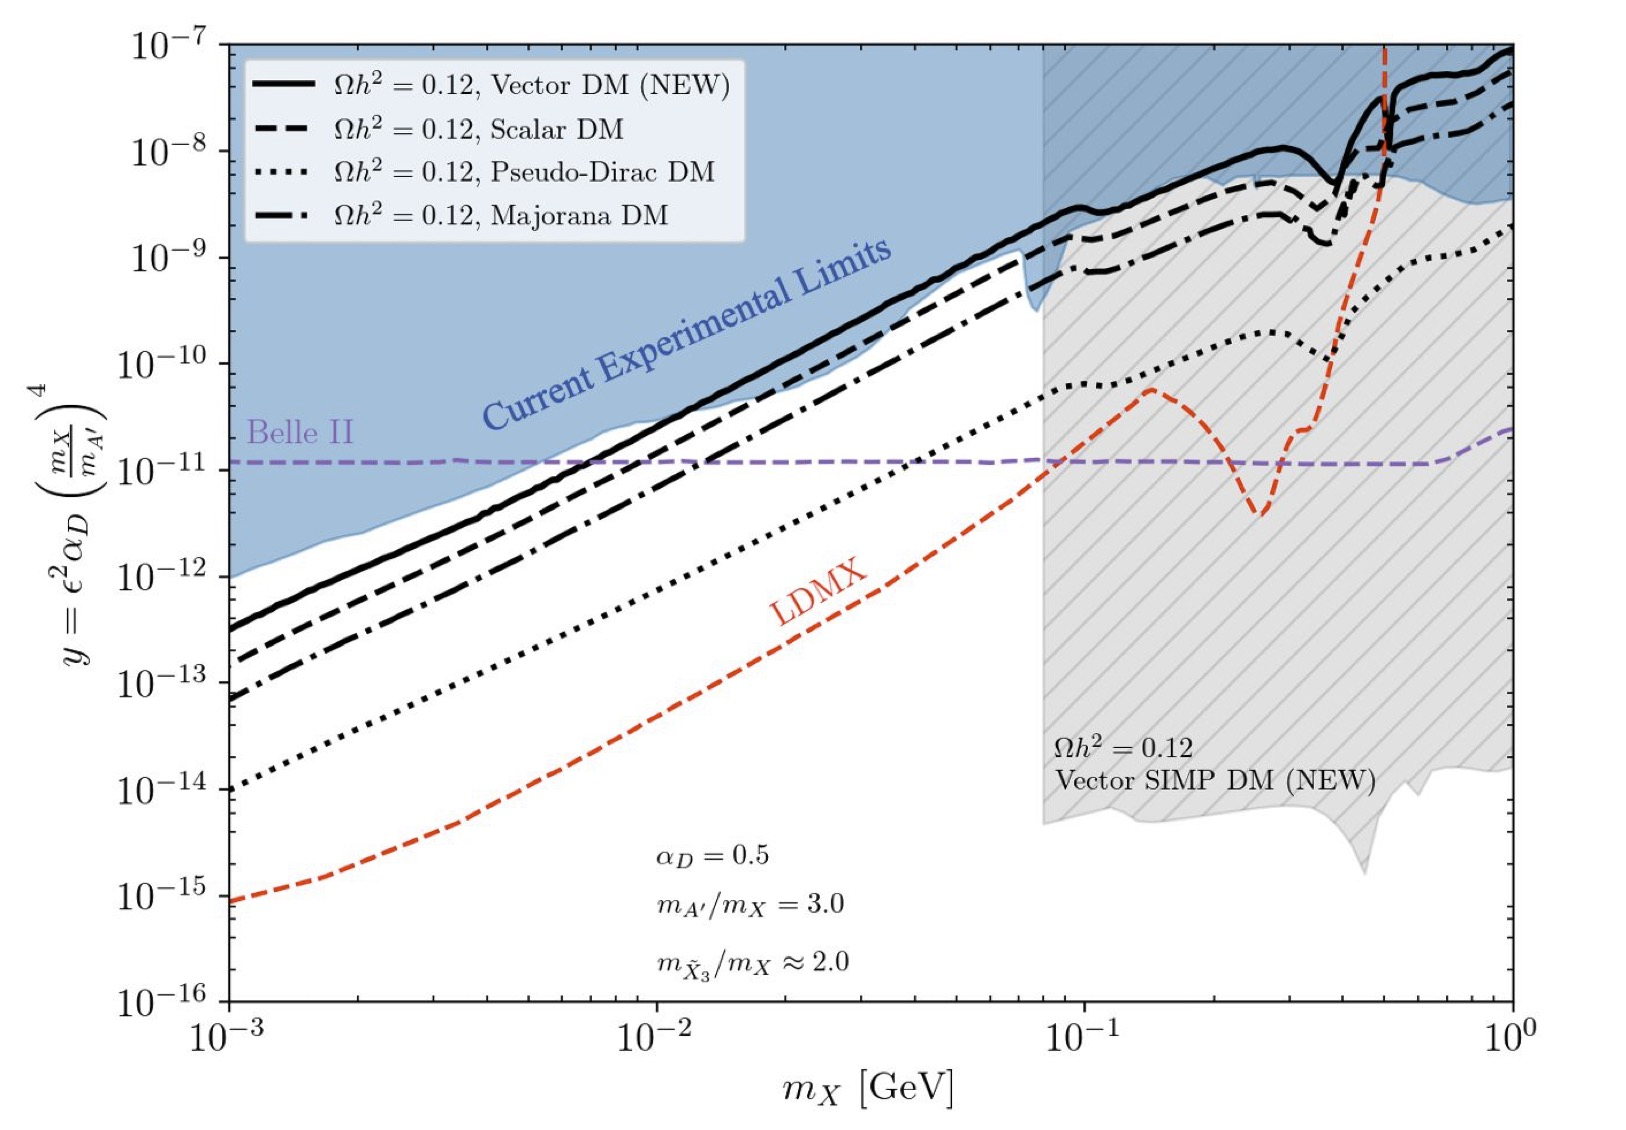
\includegraphics[width=0.80\linewidth]{config/fig/exclusion_ldmx.jpg}
    \caption{Representative comparison of thermal-relic targets with existing
    constraints and projected experimental sensitivity. The horizontal axis
    gives the dark-matter mass and the vertical axis gives the benchmark
    interaction quantity \(y\). Blue shows approximate existing constraints,
    purple shows the Belle~II projection, red shows the LDMX projection, and
    the black curves and grey region show several model-dependent \gls{dm} thermal
    targets. Reproduced from
    Refs.~\cite{catena2023-spin1-thermal-targets,ldmx2025-overview}.}
    \label{fig:exclusion_ldmx}
\end{figure}

Figure~\ref{fig:exclusion_ldmx} gives a representative view of the projected
reach. The horizontal axis shows the dark-matter mass, while the vertical
axis combines the assumed interaction strength and particle masses into the
benchmark quantity \(y\). The blue region represents parameter combinations
already constrained by earlier searches. The red curves show the smaller
interaction strengths that LDMX could test, thus expanding the frontier of 
search of \gls{dm}, while the black curves and grey
region show thermal-relic targets for several representative \gls{dm}
models. The figure is therefore a comparison within specified model
assumptions, not a model-independent exclusion of dark matter by mass alone
\cite{akesson2022-ldmx-status,catena2023-spin1-thermal-targets,
ldmx2025-overview}.

\subsubsection{Detector Layout}

Figure~\ref{fig:ldmx_detector_solid_model} shows the physical scale and
overall arrangement of the detector. The conceptual drawing in
Figure~\ref{fig:ldmx_beam_electron_schematic} illustrates the path of the
beam electron and the missing-momentum signature. The labelled cutaway in
Figure~\ref{fig:ldmx_detector_cutaway} shows the detector geometry along the
beam direction.

Two \gls{ts} modules are placed upstream of the silicon tagging tracker, and
a third is placed directly before the target. The tagging tracker measures
the incoming electron momentum. The electron then passes through the thin
tungsten target inside a dipole magnet. Its magnetic field bends charged
particles transversely according to their momentum, so a recoil electron
that has lost energy is deflected more strongly than an electron retaining
the full beam energy. A silicon recoil tracker downstream of the target
measures the momentum and direction of the outgoing charged particles.

The baseline target is \(0.1\) radiation lengths thick and has a transverse
size of \(4\,\mathrm{cm}\times10\,\mathrm{cm}\). Its small thickness limits
multiple scattering while retaining a useful production rate. The nominal
\(20\,\mathrm{mm}\times80\,\mathrm{mm}\) beam spot reduces peak detector
occupancy and helps to separate the showers from different electrons
\cite{ldmx2025-overview}.

The \gls{ecal} is placed behind the recoil tracker. It measures electrons,
photons and their shower shapes. The HCal surrounds the ECal at the sides
and rear. Its main role in the dark-matter search is to identify penetrating
hadrons and muons that could otherwise imitate missing momentum. Together,
the trackers and calorimeters measure the recoil electron and \emph{veto},
meaning reject, candidate events containing other visible particles. This
combined information distinguishes an invisible final state from ordinary
interactions in which visible particles were missed by one detector system
\cite{ldmx2025-overview}.

\begin{figure}[p]
    \centering

    \begin{minipage}[t]{0.48\linewidth}
        \vspace{0pt}
        \centering
        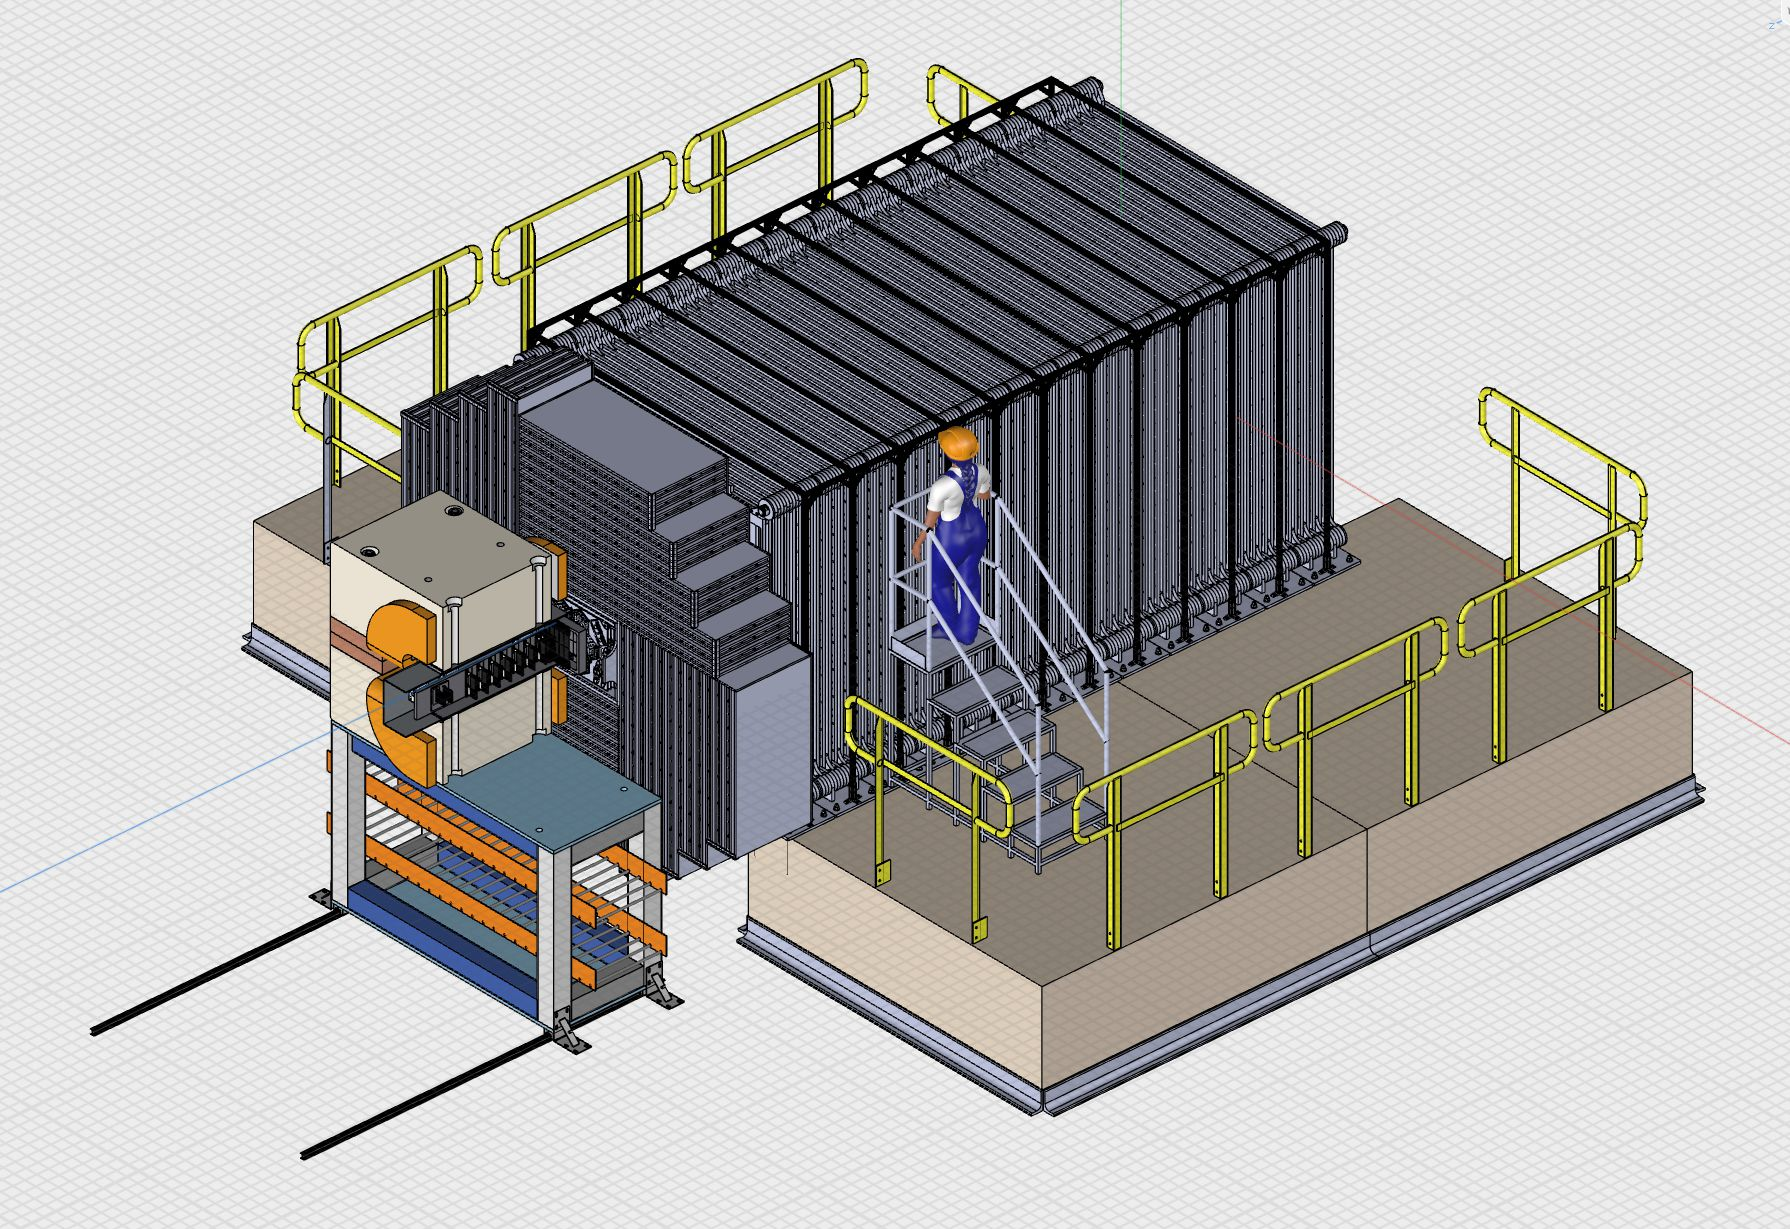
\includegraphics[
            width=\linewidth,
            height=0.20\textheight,
            keepaspectratio
        ]{config/fig/ldmx_detector_solid_model.jpg}
        \caption{Solid-model overview of the LDMX detector installation. The
        compact tracking and target region is located at the left, in front
        of the calorimeter systems. Sourced from Figure~3.1 of the 2025 LDMX
        design report \cite{ldmx2025-overview}.}
        \label{fig:ldmx_detector_solid_model}
    \end{minipage}
    \hfill
    \begin{minipage}[t]{0.48\linewidth}
        \vspace{0pt}
        \centering
        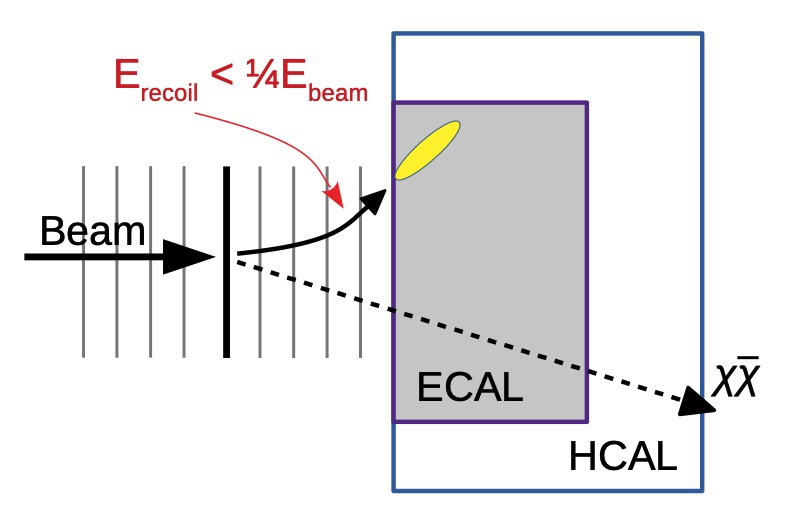
\includegraphics[
            width=\linewidth,
            height=0.20\textheight,
            keepaspectratio
        ]{config/fig/beam_electron_schematic.jpg}
        \caption{Conceptual illustration of the LDMX missing-momentum
        signature. After the beam electron passes through the tagging tracker
        and scatters in the thin tungsten target, a recoil electron carrying
        less than one quarter of the beam energy enters the ECal, while an
        invisible \(\chi\bar{\chi}\) pair carries away momentum. The ECal and
        HCal test for additional visible activity. Sourced from Figure~8 of
        the 2018 LDMX design report \cite{akesson2018-ldmx}.}
        \label{fig:ldmx_beam_electron_schematic}
    \end{minipage}

    \par\vspace{0.02\textheight}

    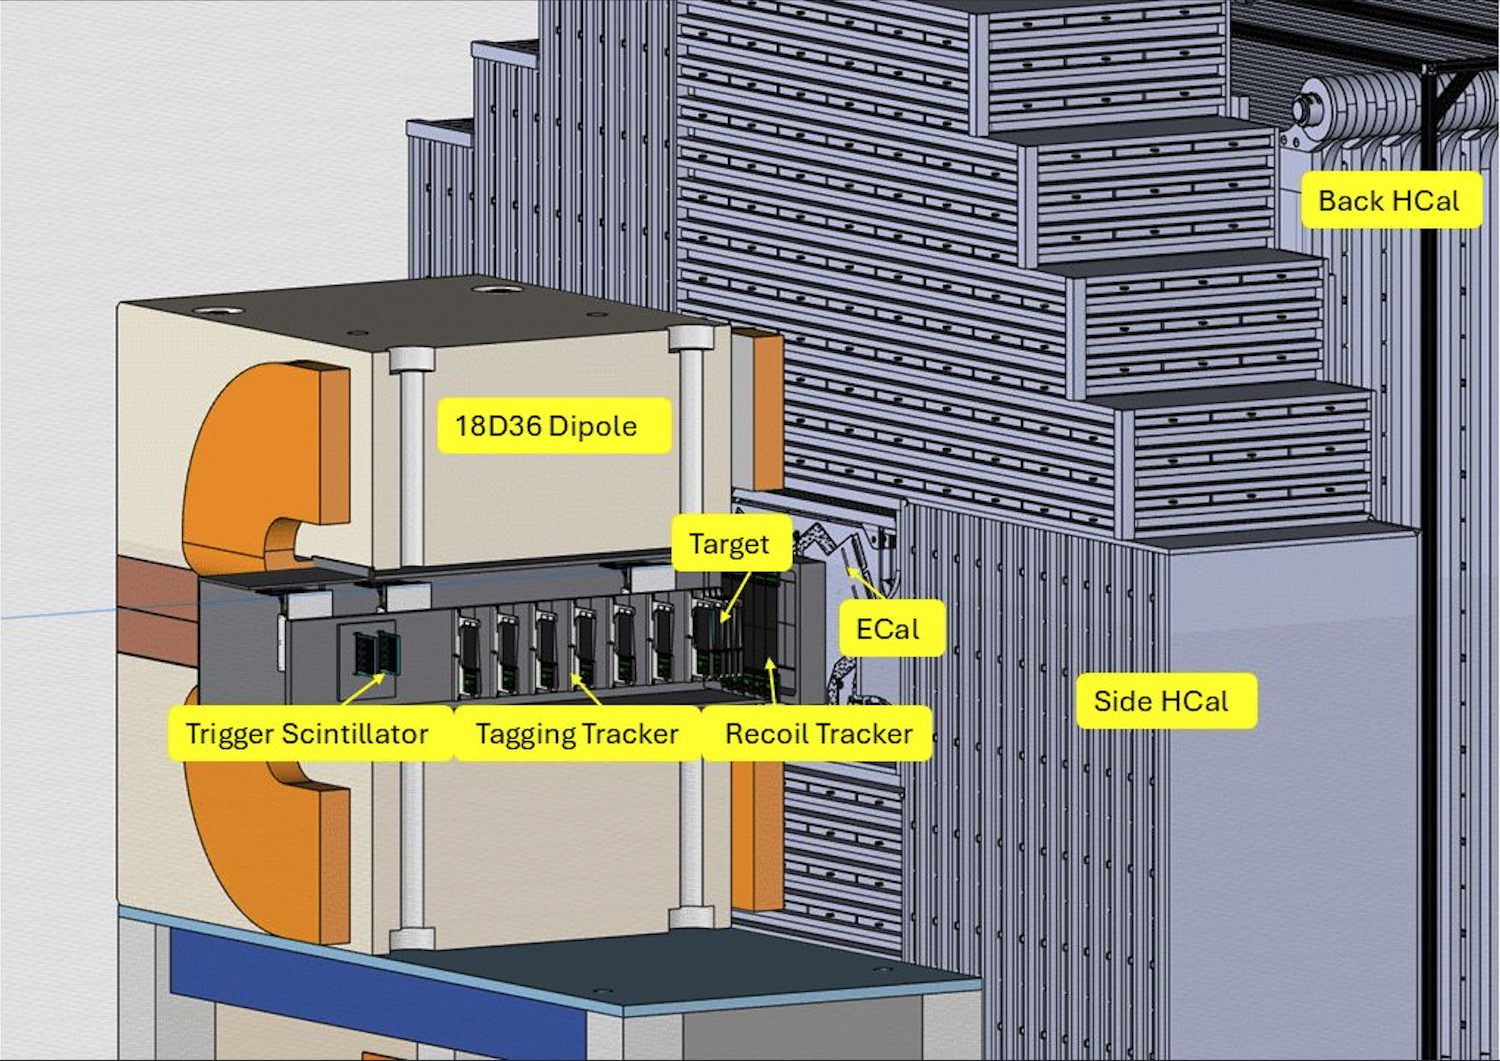
\includegraphics[
        width=\linewidth,
        height=0.47\textheight,
        keepaspectratio
    ]{config/fig/ldmx_detector_cutaway.jpg}
    \caption{Cutaway view of the LDMX detector. From left to right, it shows
    the Trigger Scintillator, tagging tracker, target inside the dipole
    magnet, recoil tracker, ECal, and the side and back HCal. Sourced from
    Figure~3.2 of the 2025 LDMX design report
    \cite{ldmx2025-overview}.}
    \label{fig:ldmx_detector_cutaway}
\end{figure}

\clearpage

\subsubsection{Electromagnetic Calorimeter and Electron Showers}

% The first section first sentence should be a 1 sentence summary what the main purpose or task with the ecal is. 
The main purpose of the \gls{ecal} is to measure the energy and spatial
development of electrons and photons, allowing the visible final state to be
reconstructed and backgrounds to be rejected. Its high-granularity 
silicon-tungsten design is a compact ''sibling detector'' of the \gls{hgcal} at the \gls{cms} experiment, from which LDMX adopts detector-module and readout technology
\cite{ldmx2025-overview}.


% This section should also mention that the ECal detector is a "sibling detector" since the design is based upon the CMS of CERN in one sentence, which a suitable reference if this info is not found in the design report. 
The ECal is a sampling calorimeter with a total depth of about \(40\)
radiation lengths. A radiation length \(X_0\) is the characteristic material
scale for energy loss by a high-energy electron through bremsstrahlung.
Tungsten layers initiate and develop electromagnetic showers, while
interleaved silicon layers sample their energy deposits. The final design
contains 32 silicon layers arranged as 16 bilayers, where each bilayer pairs
two silicon sampling planes around a common support and cooling structure.
The \path{ldmx-det-v15-8gev} geometry used in this thesis likewise produces
reconstructed ECal hits at 32 layer positions. The performance simulations in
the current (and newer) LDMX design report instead used an earlier geometry with 34
layers in 17 bilayers \cite{ldmx2025-overview}.

An energetic electron radiates photons through \gls{bremsstrahlung} as it
passes through tungsten. These photons can produce electron--positron pairs,
which radiate further photons. Repetition of these processes creates an
\gls{electron shower}. One incoming electron therefore produces energy
deposits in many cells and layers rather than a single detector hit. The energy contributions in the 3D pattern captures information about the electron position,
energy and shower development \cite{groom2024-passage-particles}.

The transverse size of an electromagnetic shower is commonly described by
the Molière radius \(R_{\mathrm{M}}\). For a homogeneous material, it is
calculated as
\begin{equation}
    R_{\mathrm{M}} = X_0\frac{E_{\mathrm{s}}}{E_{\mathrm{c}}},
    \qquad E_{\mathrm{s}} \simeq 21\,\mathrm{MeV},
    \label{eq:moliere_radius}
\end{equation}
where \(X_0\) is the radiation length, \(E_{\mathrm{s}}\) is a
material-independent scale energy, and \(E_{\mathrm{c}}\) is the critical
energy at which radiative and ionisation energy losses are comparable. On
average, about \(90\%\) of the shower energy is contained within a cylinder
of radius \(R_{\mathrm{M}}\) \cite{groom2024-passage-particles}. For the
layered \gls{ldmx} \gls{ecal}, the design report gives an effective Molière radius of
approximately \(2.5\,\mathrm{cm}\). It also reports that \(68\%\) of the
shower energy is contained within less than \(1\,\mathrm{cm}\) during
approximately the first 15 layers \cite{ldmx2025-overview}. These values
provide useful reference scales for interpreting shower overlap.

\begin{figure}[H]
    \centering
    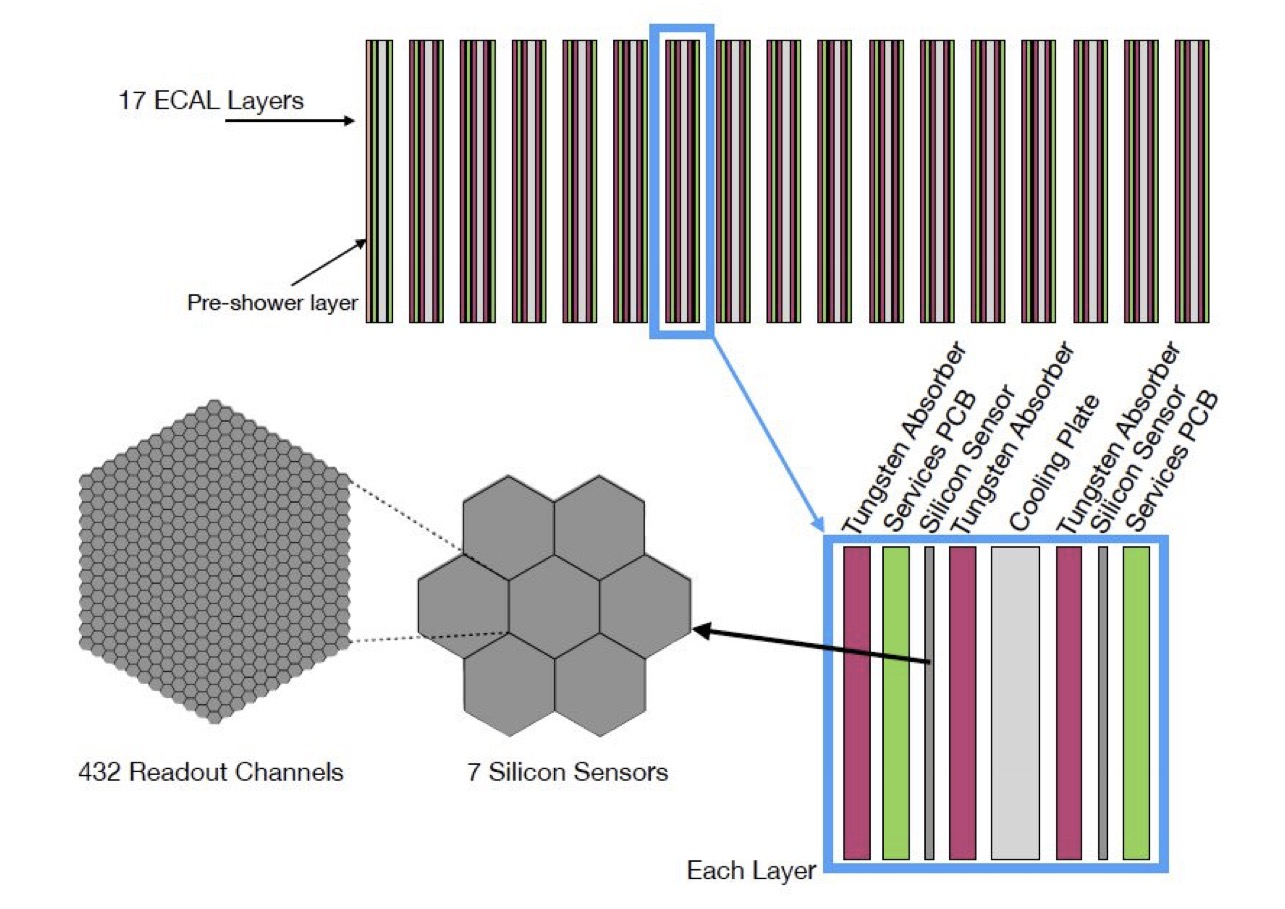
\includegraphics[width=\linewidth]{config/fig/ecal_cells_and_layers.jpg}
    \caption{Schematic of the full-resolution LDMX ECal modules and the
    components of a bilayer. Sourced from the LDMX design report \cite{ldmx2025-overview} }
    \label{fig:ecal_cells_and_layers}
\end{figure}

Each ECal sampling plane contains seven hexagonal modules, and each module
contains 432 silicon readout cells. A local cell identifier connects every
measured energy deposit with a fixed detector position.
Figure~\ref{fig:ecal_cells_and_layers} shows this full-resolution segmentation
and the bilayer construction. For the real-time trigger, groups of nine
neighbouring readout cells are summed into 48 coarser \emph{trigger cells} per
module. This grouping, which is not drawn in the figure, retains less spatial detail for the \textit{online reconstruction} compared to
the individual-cell readout available to \textit{offline reconstruction}
\cite{ldmx2025-overview}.

The fine segmentation helps separate nearby showers and identify small
energy deposits from background particles, making it central to this thesis.
When several beam electrons arrive in the same readout window, their showers
may overlap in the same layers or cells. Reconstruction must then use the
spatial and energy pattern of the full-resolution hits to determine which
electron produced each part of the event and recover per-electron shower
information from the combined response.

\subsubsection{Trigger Scintillator and Trigger-Pad Tracks}

The \gls{ts} estimates how many beam electrons enter the target in the same
readout window and where they pass through the beam region. It consists of
three modules: two directly upstream of the tagging tracker and one directly
upstream of the target. Each module contains two staggered layers of plastic
scintillator bars. A traversing electron deposits energy in a bar and produces
scintillation light that is measured as a photoelectron signal. Adjacent bar
hits are joined into clusters, and clusters across the three modules are
combined when their positions are compatible with an electron travelling
along the expected beam direction \cite{ldmx2025-overview}. Forming these
track candidates is itself a rule-based reconstruction method: low-level bar
signals are converted into estimates of electron position and multiplicity.

In this thesis, the reconstructed TS track candidates are referred to by
their name in the research-group codebase, \texttt{TriggerPadTracks}. The
term describes objects derived from TS measurements, not a separate detector,
and should not be confused as so. Each
candidate provides a one-dimensional position estimate and a photoelectron
count. Together, the candidates provide information about the positions, energy and the 
multiplicity of the incoming electrons. They are reconstructed detector
objects rather than simulation-truth labels, and correspond one-to-one with
the incident electrons only when the reconstruction makes correct prediction \cite{ldmx2025-overview}.

\subsubsection{Triggering
% and reconstruction
}
% I removed the reconstruction from the title since I think that adds reconstruction in too many titles. Reconstruction is already relevant to trigger in itself or maybe one could add a qualitatively description of the trigger that summarizes the content of this section. The trigger naturally leads into online and offline and the different resolutions one works with, and "working" with data is always reconstruction. The term reconstruction should have been defined already before this section I think? 

% We are to refine these section and simplify the description since not all of this information is relevant. Skip the description of trains that does not matter here. 

% One perspective that I have to insert here or in the next section should be that 

% Notes from supervisor: 37,14 MHz bucket, how much in nanoseconds?. beam frequency  kollimerade elektroner först i ett fåtal pikosekunder, sen finns ett 2cmx8cm fönster. 

The beam is divided into short time slots called radio-frequency buckets,
which are delivered in groups called trains. Within a train, neighbouring
buckets are separated by \(26.9\,\mathrm{ns}\), corresponding to a
\(37.14\,\mathrm{MHz}\) clock for the detector electronics. The nominal beam
structure contains 20 filled buckets in each train at a train rate of
\(1\,\mathrm{MHz}\), with an average of approximately one to two electrons
per filled bucket. 
%The estimated frequency of electrons that hit the target is ...??? \textbf{need some input from Lene-Kristian here I think} \cite{ldmx2025-overview}.

Storing the full detector response for every filled bucket is neither feasible nor desirable:
the input rate is much larger than the available readout and storage rate,
and almost all events arise from ordinary processes not displaying the benchmark interaction. 
The online trigger
therefore receives compact information from the \gls{ts}, \gls{ecal} and
\gls{hcal} at the full clock rate and decides in real time whether the complete
event should be read out and stored. The Trigger Scintillator supplies an
incoming-electron count \(n\), and the ECal supplies coarse energy sums. A
basic online estimate is
\begin{equation}
    E_{\mathrm{miss}}^{\mathrm{trig}}
    =
    nE_{\mathrm{beam}} - E_{\mathrm{ECal}}^{\mathrm{trig}} ,
\end{equation}
Here, \(E_{\mathrm{miss}}^{\mathrm{trig}}\) is the trigger-level estimate of
the missing energy, \(n\) is the number of incoming electrons estimated by
the Trigger Scintillator, and \(E_{\mathrm{beam}}\) is the nominal beam energy
per electron. The product \(nE_{\mathrm{beam}}\) therefore estimates the total
incoming energy, while \(E_{\mathrm{ECal}}^{\mathrm{trig}}\) is the energy
measured by the ECal using its coarse trigger readout. The superscript
\(\mathrm{trig}\) distinguishes quantities available to the online trigger
from those obtained through the more detailed offline reconstruction.
Over-counting the electrons can create false missing energy, while
under-counting can cause a real signal event to be rejected. The trigger
reduces the input rate to an average readout rate of about
\(10\,\mathrm{kHz}\). The primary missing-energy trigger uses part of this
bandwidth, while the remainder supports other physics, calibration and
monitoring selections \cite{ldmx2025-overview}.

The distinction between online and offline reconstruction is set by this
decision. Online reconstruction occurs before storage and must satisfy strict
limits on latency, memory and transferred information. It therefore uses
reduced quantities such as ECal trigger-cell sums and Trigger Scintillator
track candidates. Once an accepted event has been fully read out, offline
reconstruction (which techincally has no deadline) can use individual ECal cells and more computationally
demanding algorithms to construct calibrated hits, tracks, showers and
analysis quantities \cite{ldmx2025-overview}.


The methods developed in this thesis use simulated ECal hits at the full cell
granularity, together with reconstructed trigger-pad tracks. They
therefore belong to offline reconstruction research. Their results can show
whether electron showers can be separated under multi-electron conditions.
Deployment in the online trigger would be a separate task because it would
require reduced trigger inputs and a dedicated latency and hardware study.

\subsubsection{Pile-Up, Reconstruction and Physics Reach}
\label{sec:formalism}
% This section is a bit all over the place, it has to be tightened and get a good logical flow. All information that I want to give is contained here it needs to be presented in the best format possibly simply. 

% This section contains too much in one place. It should be broken up where pile-up is one section



% Notes from my supervisor discussion: Multipliciteten beskrivs i en poissonfördelning och den är relativt bred så $\mu = 1$ ger också 2 och 3 elektroner. => det gör att endast $37\%$ av händelserna kan användas







In this thesis, \gls{pile-up} mainly refers to \emph{in-time pile-up}, where
two or more beam electrons arrive in the same time sample and their detector
responses are recorded together. 
\textbf{True?: Trigger latency does not create in-time pile-up. It follows from the number of electrons delivered in the same bucket.}
Lowering the beam intensity would reduce it, but would also
reduce the number of \gls{eot} accumulated per unit time. The practical
challenge is therefore to retain the advantages of higher beam intensity
without losing events because their detector responses are combined
\cite{ldmx2025-overview}.

% The approximation/assumption of independent electron propagation should be mentioned here, but I should also say that one is allowed to this to a very good approximation single electrons are abbysmal low chances of colliding or affecting each other. It is very handy that the eletrons can be approximated as independent since that simplifies computation nicely. 
To a very good approximation, separate beam electrons propagate
independently: the probability that two beam electrons interact directly with
each other is negligible. This simplifies simulation as their propagations 
can be simulated independently and then \emph{overlayed} before simulating their detector responses. Let
\(Z^{(k)}\) denote the true ECal energy-deposition pattern from source
electron \(k\).  Under this simulation assumption,
\begin{equation}
    Z^{(k)} \perp\!\!\!\perp Z^{(\ell)}
    \qquad \text{for } k\neq\ell .
\end{equation}
After overlay and detector reconstruction, the observed hit collection from the detectors is a
combined response,
\begin{equation}
    \mathcal{H}
    =
    \mathcal{R}\!\left(
        Z^{(1)},\ldots,Z^{(m)}
    \right).
\end{equation}
The response \(\mathcal{R}\) is a nondeterministic mapping that includes detector granularity, thresholds,
noise and hit reconstruction. Deposits from different electrons may then
occupy the same cell or form overlapping showers. The observed collection
\(\mathcal{H}\) cannot in general be divided into its original components $Z^{(1)},\ldots,Z^{(m)}$ by
a simple geometric cut.

The overlap affects both triggering and later analysis. An
incorrect electron count can produce an incorrect missing-energy estimate.
Overlapping showers also make the ECal topology harder to interpret and can
cover small deposits that are needed to reject backgrounds. The trigger must
therefore use thresholds that depend on the estimated electron count.
Offline reconstruction can use the full stored detector response to determine
which multi-electron events remain separable and how much per-electron
information can be recovered. Such studies can later inform which event
classes are useful enough to retain at trigger level, although deploying an
online method requires a separate trigger study. This thesis addresses the
offline problem by assigning the combined ECal activity to the different beam
electrons \cite{ldmx2025-overview}.

Multi-electron events are also an opportunity. The design report estimates
that \(4\times10^{14}\) \gls{eot} can be accumulated in about twelve months
with an average of one electron per sample. Reaching exposures of order
\(10^{16}\) \gls{eot} efficiently requires higher beam intensity and the
ability to use events containing several electrons. In a design study with
an average multiplicity \(\mu=1\), accepting up to four reconstructed
Trigger Scintillator tracks instead of only one increased the total signal
trigger efficiency from \(0.58\) to \(0.88\) at approximately the same
\(1\,\mathrm{kHz}\) trigger budget. This result used a
\(0.1\,\mathrm{GeV}\) dark-photon benchmark and the energy in the first 20
ECal layers \cite{ldmx2025-overview}.

% TODO: Add the supervisor's running-time estimate only after the assumed
% beam intensity, target, one-electron selection and personal-communication
% citation have been specified.

Rejecting every multi-electron sample would discard part of the delivered
beam and extend the time needed to reach a given exposure. If overlapping
showers can instead be reconstructed reliably, more recorded events become
useful and the intended sensitivity can be reached sooner. This is how
pile-up handling can increase the practical physics reach of LDMX.

The specific problem studied in this thesis is a step towards that goal. The
study considers two-electron and three-electron events as direct extensions
of the single-electron case; higher multiplicities are outside its scope. The
samples are constructed from independent single-electron simulations, and
the models attempt to assign ECal hits to their electron of origin. The study
does not itself search for \gls{dm}. It tests whether modern reconstruction
methods can recover per-electron shower structure from the combined detector
response produced by multi-electron operation.



\subsection{Machine Learning Methods for Reconstruction in High Energy Physics}
\label{sec:ml_event_reconstruction_hep}


Short introductory text here stating that ML is a topic of rising interest in HEP and refer to output of ML-related papers in HEP. \cite{iml-wg-hepml-livingreview}'. \textbf{I have realized that the relevancy of this section is heavily questioned... Just cherry-pick relevant parts from here and ommit the rest I have limited space and this is not a popular science summary this background should cover necessary theory and it should cover necessary motivation for my study in my thesis, and maybe provide some context for the viewer also but nothing else. The fact that it is a rising tool of interest is still interesting to mention, but only in the contexts of why that is not simply a ''trend follower''. The rising tool of interest should be 1 or max 2 sentences.}


\textbf{text here}

\gls{ml} has become a tool of rising interest in \gls{hep}, driven by the growing complexity of detector data, the need for efficient event selection, and the search for rare signatures of physics beyond the \gls{sm}. At the same time, advances in deep-learning methods and accelerator-based computing architectures such as \glspl{gpu} have made increasingly powerful \gls{ml} and non-\gls{ml} approaches practical for scientific workflows \cite{sur2026-heterogeneous-computing}. Machine learning and deep-learning methods are not new in \gls{hep}, but the recent rapid growth of machine-learning applications in particle physics is 
\begin{wrapfigure}{r}{0.50\textwidth}
    \centering
    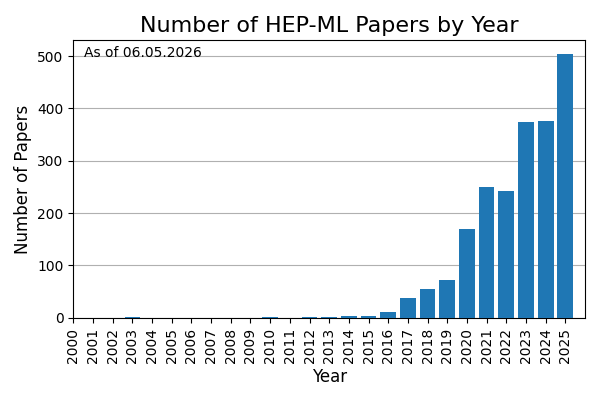
\includegraphics[width=0.48\textwidth]{config/fig/per_year.png}
    \caption{\textbf{Increase the size of labels here} Number of machine-learning-related publications on arXiv in the HEP category per year, based on the Living Review of Machine Learning for Particle Physics \cite{iml-wg-hepml-livingreview}.}
    \label{fig:ml-publications-per-year}
\end{wrapfigure}
reflected both in dedicated reviews and in the continuously updated Living Review of Machine Learning for Particle Physics  \cite{karagiorgi2021-mlnewphysics,feickert2021-livingreview,iml-wg-hepml-livingreview}. Figure \ref{fig:ml-publications-per-year} shows the trend of machine-learning-related publications within \gls{hep} significantly increasing in the last few years. 


The underlying motivation for \gls{ml} in \gls{hep} is that such tools may increase the \textit{physics reach} of experiments, meaning their ability to probe weaker signals, rarer processes, or more challenging regions of parameter space, either by improving sensitivity enabling new discoveries or by making reconstruction and selection more computationally efficient. 

\paragraph{Reconstruction} Reconstruction in \gls{hep} refers to reconstructing the physical interpretables from a measured particle event based on the detector outputs.  Modern \gls{hep} experiments produce high-dimensional and heterogeneous data, where each event may contain a variable number of detector signals distributed across several subdetectors. This makes reconstruction a quite natural application area for machine learning: the task is to transform heterogeneous low-level or intermediate detector information, such as hits, tracks, and calorimeter clusters, into physically meaningful quantities that can be used for triggering, event selection, and analysis.



A useful way to view reconstruction is as an approximate inverse problem. In simulation, a detector may be regarded as a map from an underlying particle-level event to a set of detector measurements. If the particle-level event, representing the physical ''truth'', is denoted by \(Y\), and the corresponding detector response by \(X\), the simulation can be written schematically as
\begin{equation}
    S(Y) = X ,
\end{equation}
where \(S\) represents the detector response. Reconstruction, denoted $R$,  then attempts to inverse the mapping, i.e
\begin{equation}
    R(X) \approx S^{-1}(X) = Y .
\end{equation}
In practice, this inverse is imperfect and often ambiguous, based on the fact that some information is always lost, has stochastic evolutions or only indirectly observed: detector signals have finite resolution and particles may overlap in the detector. These cases does not exclude relevance however, as it could also be useful to study these scenarios as well and infer where our tools of measurement might simply not be enough. Machine-learning-based reconstruction approaches formulate parts of this inverse problem as a learnable mapping from detector-level inputs to physics-level targets, typically using simulated events where truth information is available to us and constructing target information is completely feasible.

\subsubsection{Computational Context in Experimental High Energy Physics}

The computational setting of \gls{hep} is also important for understanding the interest in machine-learning-based reconstruction. Large-scale \gls{hep} computing has traditionally been dominated by distributed, \gls{cpu}-based workflows. \cite{sur2026-heterogeneous-computing} This is natural because collision or fixed-target events often are, to a good approximation, independent processes, analog to the electron case of \gls{ldmx} $Z^{(k)} \perp\!\!\!\perp Z^{(\ell)}$ where $k \neq l$, following the notation introduced in Section~\ref{sec:formalism}. Simulation, reconstruction, and analysis can therefore often be parallelized over events with relatively little communication between tasks, making \gls{cpu} clusters and grid computing highly effective, somewhat bypassing an immediate need of software engineering concurrency, which explains the longevity and success of this computing paradigm within \gls{hep}.

At the same time, the wider computing landscape has shifted toward heterogeneous architectures, in particular \glspl{gpu} and other accelerator \footnote{``Accelerator'' in this context refers to specialized hardware such as \glspl{gpu} or even \gls{ml} specialized architectures such as the relatively new \gls{tpu} designed by Google that accelerate the speed of computation for applicable processes\cite{needed}}
-based systems. This development is strongly connected to modern machine learning, where many operations reduce to dense linear algebra and can be executed efficiently on massively parallel hardware, including both training and inference tasks of deep learning \gls{ml} models.

This shift creates both a challenge and an opportunity for \gls{hep}. Rule-based reconstruction algorithms have often been designed around detector-specific logic and sequential or iterative procedures. Such algorithms can be highly effective, but they may be difficult to port efficiently to accelerator hardware and may scale poorly with detector occupancy. Machine-learning models, by contrast, often express reconstruction as a fixed sequence of tensor operations, making inference naturally suited to \glspl{gpu} or other accelerator architectures. 

\subsubsection{MLPF, a Recent Example of ML-based Reconstruction in HEP}

\gls{mlpf}, developed for the \gls{cms} experiment, provides a relevant
example of machine learning used inside reconstruction rather than only as a
final event classifier. The original study used a graph-neural-network
architecture for particle-flow reconstruction in high-pile-up conditions
\cite{pata2021-mlpf}. A later implementation uses a Transformer architecture
integrated into the CMS reconstruction software and evaluates it on both
simulation and collision data \cite{pata2026-mlpf}. The transition also
illustrates the growing importance of accelerator-friendly computation for
high-dimensional, variable-size event data.

Machine-learning and rule-based reconstruction are complementary rather than
exclusive. MLPF receives detector objects that already include outputs from
earlier reconstruction stages, then learns associations and particle-level
predictions from those objects. The present thesis studies a narrower
LDMX-specific problem---separating overlapping electron showers at hit
level---but adopts the same general view of an event as a variable-size
collection of heterogeneous detector objects.

\subsubsection{Detector Events as Unordered Sets}
\label{sec:detector_set_background}

Under pile-up, several particles can contribute to nearby or even identical
detector cells. Reconstruction must therefore use the pattern formed by many
detector objects, rather than classify each hit from its own features alone.
For one event, these objects can be written as a variable-size set
\begin{equation}
    \mathcal{X}
    =
    \{\mathbf{x}_1,\ldots,\mathbf{x}_N\},
\end{equation}
where \(\mathbf{x}_i\) contains the measured features of one ECal hit or
trigger-pad track. The storage index \(i\) has no physical meaning.

This representation avoids projecting the three-dimensional ECal and the
different trigger-pad objects onto one regular image. A convolutional neural
network is naturally biased towards a fixed grid and local translation
symmetry, whereas the number and geometry of detector objects vary between
events. Graph neural networks and Transformer encoders instead retain every
object as a node or token and learn how the objects should exchange
information \cite{duarte2020-gnn-tracking,lee2019-set-transformer}.

For the per-object models used here, reordering the input should only reorder
the corresponding outputs. If \(\mathbf{P}\) is a permutation matrix and
\(\mathbf{F}\) denotes the network, this requirement is
\begin{equation}
    \mathbf{F}(\mathbf{P}\mathbf{X})
    =
    \mathbf{P}\mathbf{F}(\mathbf{X}).
\end{equation}
Both GravNet and a Transformer encoder without sequence-position encodings
have this permutation-equivariant property. Their principal difference is
how they choose the other objects from which each node or token receives
information.

\subsubsection{Graph Neural Networks and GravNet}
\label{sec:gnn_gravnet_background}

A graph represents detector objects as nodes and the permitted information
exchanges as edges. A GNN layer performs the same operation for every node: it
collects messages from the node's neighbours and uses their sum to update the
node representation. The standard message-passing formulation is
\begin{align}
    \mathbf{m}_i^{(\ell)}
    &=
    \sum_{j\in\mathcal{N}(i)}
    M^{(\ell)}\!\left(
        \mathbf{h}_i^{(\ell)},
        \mathbf{h}_j^{(\ell)},
        \mathbf{e}_{ij}
    \right),
    \label{eq:generic_message}\\
    \mathbf{h}_i^{(\ell+1)}
    &=
    U^{(\ell)}\!\left(
        \mathbf{h}_i^{(\ell)},
        \mathbf{m}_i^{(\ell)}
    \right).
    \label{eq:generic_update}
\end{align}
Here, \(\mathbf{h}_i^{(\ell)}\) is the representation of node \(i\) in layer
\(\ell\), \(\mathcal{N}(i)\) is its set of neighbours, and
\(\mathbf{e}_{ij}\) denotes optional information about their connecting edge.
The learned function \(M\) constructs one message from each neighbour and the
learned function \(U\) combines their sum with the current node. In intuitive
terms, the first line asks ``what do my neighbours tell me?'', while the second
asks ``how should that information change me?'' The sum is independent of
neighbour order. Other GNNs may replace it with a mean or maximum, but the
principle is unchanged \cite{gilmer2017-message-passing,duarte2020-gnn-tracking}.

\glsunset{gravnet}
GravNet differs from a GNN with a fixed graph because it learns which nodes
should be neighbours. In every GravNet layer, each node representation
\(\mathbf{h}_i\) is first mapped to two learned quantities:
\begin{align}
    \mathbf{s}_i &= \mathbf{W}_s\mathbf{h}_i+\mathbf{b}_s,
    &
    \mathbf{f}_i &= \mathbf{W}_f\mathbf{h}_i+\mathbf{b}_f.
    \label{eq:gravnet_projections}
\end{align}
The matrices \(\mathbf{W}\) and biases \(\mathbf{b}\) are learned during
training. The coordinate \(\mathbf{s}_i\) determines who the neighbours are,
whereas \(\mathbf{f}_i\) contains the information that node \(i\) can send.
Importantly, \(\mathbf{s}_i\) is not a physical detector position; it is an
internal coordinate chosen by the network for the prediction task.

Each node is connected to the \(k\) nodes with the smallest Euclidean distance
in this learned space. Information from a neighbour \(j\) is then weighted as
\begin{align}
    d_{ij}^{2}
    &= \lVert\mathbf{s}_i-\mathbf{s}_j\rVert_2^2,
    &
    \mathbf{m}_{j\rightarrow i}
    &= \underbrace{\exp(-\lambda d_{ij}^{2})}_{\text{distance weight}}
       \mathbf{f}_j.
    \label{eq:gravnet_message}
\end{align}
The original GravNet paper uses the Gaussian potential with \(\lambda=1\)
\cite{qasim2019-gravnet}; the PyTorch Geometric implementation
\cite{fey2019-pytorch-geometric} used here sets \(\lambda=10\). In either case,
the interpretation is simple: a nearby node in the learned space contributes
strongly, while a distant node contributes little.

Finally, the incoming messages are reduced to fixed-size summaries and used to
update the node:
\begin{align}
    \mathbf{a}_i
    &=
    \left[
        \underset{j\in\mathcal{N}_k(i)}{\operatorname{mean}}
        \mathbf{m}_{j\rightarrow i}
        \,\middle\Vert\,
        \underset{j\in\mathcal{N}_k(i)}{\operatorname{max}}
        \mathbf{m}_{j\rightarrow i}
    \right],
    \label{eq:gravnet_aggregation}\\
    \mathbf{h}'_i
    &=
    \mathbf{W}_{\mathrm{self}}\mathbf{h}_i
    +
    \mathbf{W}_{\mathrm{agg}}\mathbf{a}_i
    +\mathbf{b}.
    \label{eq:gravnet_update}
\end{align}
The maximum is taken element by element and \(\Vert\) denotes concatenation.
Intuitively, the mean describes the typical neighbour message, the maximum
retains its strongest components, and the first term in the update preserves
information from the node itself. A new neighbour graph is constructed in
every layer, so the network can learn a different notion of similarity at
each stage. Figure~\ref{fig:gravnet_convolution} visualises the same sequence.

\begin{figure}[htbp]
    \centering
    \resizebox{0.99\linewidth}{!}{%
    \begin{tikzpicture}[
        >=Latex,
        every node/.style={font=\small},
        block/.style={
            draw,
            rounded corners,
            align=center,
            minimum height=11mm,
            text width=25mm,
            inner sep=2pt,
            fill=RoyalBlue!8
        },
        learned/.style={
            block,
            fill=ForestGreen!11
        },
        operation/.style={
            block,
            text width=24mm,
            fill=ForestGreen!11
        },
        graphnode/.style={
            circle,
            draw=ForestGreen!70!black,
            fill=ForestGreen!18,
            minimum size=5mm,
            inner sep=0pt
        },
        targetnode/.style={
            graphnode,
            draw=Orange!80!black,
            fill=Orange!35,
            very thick
        },
        arrow/.style={->, thick},
        graph/.style={ForestGreen!65!black, thick},
        residual/.style={->, thick, dashed, RoyalBlue!75!black}
    ]
        \node[block] (input) at (-6.2,0)
            {current node\\representations \(\mathbf{h}_i\)};
        \node[learned] (coords) at (-3.75,1.25)
            {learned coordinates\\\(\mathbf{s}_i=\mathbf{W}_s\mathbf{h}_i+\mathbf{b}_s\)};
        \node[learned] (features) at (-3.75,-1.25)
            {propagated features\\\(\mathbf{f}_i=\mathbf{W}_f\mathbf{h}_i+\mathbf{b}_f\)};

        \draw[rounded corners, fill=ForestGreen!4, draw=ForestGreen!55!black]
            (-2.05,0.15) rectangle (1.15,2.35);
        \node[font=\small\bfseries] at (-0.45,2.05)
            {learned \(k\)-NN graph};
        \node[targetnode] (gi) at (-0.45,1.12) {\(i\)};
        \node[graphnode] (g1) at (-1.55,1.67) {};
        \node[graphnode] (g2) at (0.55,1.75) {};
        \node[graphnode] (g3) at (-1.35,0.55) {};
        \node[graphnode] (g4) at (0.65,0.55) {};
        \draw[graph, ->] (g1) -- (gi);
        \draw[graph, ->, line width=1.1pt] (g2) -- (gi);
        \draw[graph, ->, line width=1.7pt] (g3) -- (gi);
        \draw[graph, ->, line width=0.7pt] (g4) -- (gi);

        \node[operation] (messages) at (2.85,0)
            {distance-weighted messages\\
             \(\mathbf{m}_{j\rightarrow i}=w_{ij}\mathbf{f}_j\)\\[-1mm]
             {\scriptsize \(w_{ij}=e^{-10d_{ij}^{2}}\)}};
        \node[operation] (aggregate) at (5.75,0)
            {element-wise\\mean and maximum\\
             \([\mathbf{a}^{\mathrm{mean}}_i
             \Vert\mathbf{a}^{\mathrm{max}}_i]\)};
        \node[block, text width=21mm] (output) at (8.35,0)
            {updated node\\representation \(\mathbf{h}'_i\)};
        \node[block] (self) at (2.85,-2.0)
            {linear transform of\\the original \(\mathbf{h}_i\)};

        \draw[arrow] (input) -- (coords);
        \draw[arrow] (input) -- (features);
        \draw[arrow] (coords) -- (-2.05,1.25);
        \draw[arrow] (1.15,1.25) -| (messages.north);
        \draw[arrow] (features) -- (messages);
        \draw[arrow] (messages) -- (aggregate);
        \draw[arrow] (aggregate) -- (output);
        \draw[residual] (input.south) |- (self.west);
        \draw[residual] (self.east) -| (output.south);
    \end{tikzpicture}%
    }
    \caption{Data flow through one \texttt{GravNetConv} operation. Each node
    is projected into a learned coordinate space and connected to its
    \(k\) nearest neighbours within the event. Neighbour features are weighted
    by learned-space distance, aggregated by their element-wise mean and
    maximum, and combined with a transformed copy of the original node.
    Original diagram based on the GravNet operation introduced in
    Ref.~\cite{qasim2019-gravnet}.}
    \label{fig:gravnet_convolution}
\end{figure}


The models in this thesis use either \gls{ecal} hits alone or \gls{ecal} hits
and trigger-pad tracks as nodes. A stack of \texttt{GravNetConv} layers
returns one representation per node, and a shared output head produces the
per-node predictions. Only ECal-node outputs are supervised for the
hit-origin task. Once the neighbour graph has been found, message aggregation
uses \(Nk\) directed neighbour relations rather than all \(N^2\) node pairs;
the cost of the \(k\)-nearest-neighbour search is additional and depends on
its implementation. The exact dimensions and residual block structure are
given in Section~\ref{sec:method_models}.

\subsubsection{Transformer Encoders and Self-Attention}
\label{sec:transformer_encoder_background}

A Transformer calls each input object a \emph{token}; in this thesis, a token
is an ECal hit or trigger-pad track. A shared input projection maps every
feature vector \(\mathbf{x}_i\) to
\(\mathbf{h}_i\in\mathbb{R}^{d_{\mathrm{model}}}\). For an event with \(N\)
tokens, the representations form
\(\mathbf{H}\in\mathbb{R}^{N\times d_{\mathrm{model}}}\).

Self-attention updates a token by forming a weighted combination of all valid
tokens in the same event. For one attention head, learned linear projections
produce a query, key and value for every token:
\begin{equation}
    \mathbf{Q}=\mathbf{H}\mathbf{W}_Q,
    \qquad
    \mathbf{K}=\mathbf{H}\mathbf{W}_K,
    \qquad
    \mathbf{V}=\mathbf{H}\mathbf{W}_V.
    \label{eq:transformer_qkv}
\end{equation}
The query \(\mathbf{q}_i\) expresses what token \(i\) seeks, the key
\(\mathbf{k}_j\) describes what token \(j\) offers for matching, and the value
\(\mathbf{v}_j\) contains the information that token \(j\) can send. The
attention weights and updated representation are
\begin{align}
    \alpha_{ij}
    &=
    \frac{
        \exp(\mathbf{q}_i^{\mathsf T}\mathbf{k}_j/\sqrt{d_k})
    }{
        \sum_{m=1}^{N}
        \exp(\mathbf{q}_i^{\mathsf T}\mathbf{k}_m/\sqrt{d_k})
    },
    &
    \mathbf{z}_i
    &=
    \sum_{j=1}^{N}\alpha_{ij}\mathbf{v}_j ,
    \label{eq:token_attention}
\end{align}
where \(d_k\) is the query and key dimension. In matrix form
\cite{vaswani2017attention},
\begin{equation}
    \operatorname{Attention}(\mathbf{Q},\mathbf{K},\mathbf{V})
    =
    \operatorname{softmax}
    \!\left(
        \frac{\mathbf{Q}\mathbf{K}^{\mathsf{T}}}{\sqrt{d_k}}
    \right)
    \mathbf{V},
    \label{eq:scaled_dot_product_attention}
\end{equation}
Each row of \(\boldsymbol{\alpha}\) sums to one.
Thus, every updated token is a learned weighted average of information from
the complete event, not merely from nearby detector cells.

Multi-head attention repeats this calculation with independent projections.
The head outputs are concatenated and linearly mixed, allowing different
heads to represent different object-to-object relations. The reported models
use a pre-layer-normalized encoder block,
\begin{align}
    \widetilde{\mathbf{H}}
    &=
    \mathbf{H}
    +
    \operatorname{MHA}\!\left(\operatorname{LN}(\mathbf{H})\right),
    \label{eq:preln_attention}\\
    \mathbf{H}'
    &=
    \widetilde{\mathbf{H}}
    +
    \operatorname{FFN}\!\left(
        \operatorname{LN}(\widetilde{\mathbf{H}})
    \right),
    \label{eq:preln_ffn}
\end{align}
where \(\operatorname{FFN}\) is the same two-layer feed-forward network
applied independently to every token. The additions are residual connections,
which preserve an unchanged path for the previous representation. Stacking
encoder blocks alternates global information exchange with token-wise
non-linear processing. Figure~\ref{fig:transformer_encoder} shows both the
attention update and the pre-layer-normalized block used in this thesis.

\begin{figure}[htbp]
    \centering
    \resizebox{0.98\linewidth}{!}{%
    \begin{tikzpicture}[
        >=Latex,
        every node/.style={font=\small},
        block/.style={
            draw,
            rounded corners,
            align=center,
            minimum height=10mm,
            text width=25mm,
            inner sep=2pt,
            fill=RoyalBlue!8
        },
        projection/.style={
            block,
            text width=16mm,
            fill=Orange!14
        },
        operation/.style={
            block,
            text width=29mm,
            fill=Orange!14
        },
        layer/.style={
            draw,
            rounded corners,
            align=center,
            minimum height=9mm,
            text width=17mm,
            inner sep=2pt,
            fill=RoyalBlue!8
        },
        add/.style={
            circle,
            draw,
            fill=white,
            minimum size=7mm,
            inner sep=0pt
        },
        arrow/.style={->, thick},
        residual/.style={->, thick, dashed, RoyalBlue!75!black}
    ]
        \node[font=\normalsize\bfseries] at (0,2.75)
            {(a) Multi-head self-attention};

        \node[block] (hidden) at (-6.0,0.75)
            {event tokens\\\(\mathbf{H}\in\mathbb{R}^{N\times d}\)};
        \node[projection] (query) at (-3.65,1.55)
            {query\\\(\mathbf{Q}\)};
        \node[projection] (key) at (-3.65,0.75)
            {key\\\(\mathbf{K}\)};
        \node[projection] (value) at (-3.65,-0.05)
            {value\\\(\mathbf{V}\)};
        \node[operation] (weights) at (-0.65,1.15)
            {compare every token pair\\
             scaled dot products\\
             row-wise softmax \(\rightarrow\boldsymbol{\alpha}\)};
        \node[operation] (weighted) at (3.05,0.75)
            {weighted information\\[-1mm]
             \(\mathbf{Z}=\boldsymbol{\alpha}\mathbf{V}\)};
        \node[block, text width=22mm] (heads) at (6.25,0.75)
            {repeat over heads,\\concatenate and project};

        \draw[arrow] (hidden) -- (query);
        \draw[arrow] (hidden) -- (key);
        \draw[arrow] (hidden) -- (value);
        \draw[arrow] (query) -- (weights);
        \draw[arrow] (key) -- (weights);
        \draw[arrow] (weights) -- (weighted);
        \draw[arrow] (value) -- (weighted);
        \draw[arrow] (weighted) -- (heads);

        \draw[RoyalBlue!35, thick] (-7.25,-0.75) -- (7.25,-0.75);

        \node[font=\normalsize\bfseries] at (0,-1.35)
            {(b) One pre-layer-normalized encoder block};

        \node[layer] (hin) at (-6.3,-3.15)
            {input\\\(\mathbf{H}^{(\ell)}\)};
        \node[layer] (lnone) at (-4.35,-3.15)
            {LayerNorm};
        \node[layer, fill=Orange!14] (mha) at (-2.25,-3.15)
            {multi-head\\attention};
        \node[add] (addone) at (-0.25,-3.15) {\(+\)};
        \node[layer] (lntwo) at (1.65,-3.15)
            {LayerNorm};
        \node[layer, fill=Orange!14] (ffn) at (3.75,-3.15)
            {token-wise\\feed-forward};
        \node[add] (addtwo) at (5.65,-3.15) {\(+\)};
        \node[layer] (hout) at (7.2,-3.15)
            {output\\\(\mathbf{H}^{(\ell+1)}\)};

        \draw[arrow] (hin) -- (lnone);
        \draw[arrow] (lnone) -- (mha);
        \draw[arrow] (mha) -- (addone);
        \draw[arrow] (addone) -- (lntwo);
        \draw[arrow] (lntwo) -- (ffn);
        \draw[arrow] (ffn) -- (addtwo);
        \draw[arrow] (addtwo) -- (hout);
        \draw[residual] (hin.north) -- ++(0,0.75) -|
            node[pos=0.25, above, font=\scriptsize] {residual}
            (addone.north);
        \draw[residual] (addone.south) -- ++(0,-0.75) -|
            node[pos=0.25, below, font=\scriptsize] {residual}
            (addtwo.south);
    \end{tikzpicture}%
    }
    \caption{Transformer operations used in this thesis. Panel (a) shows how
    one attention head compares every valid token pair and forms a weighted
    mixture of their value vectors; several heads repeat the operation with
    independent projections. Panel (b) shows the pre-layer-normalized encoder
    block used by the reported models. Diagram conventions are adapted from
    NNTikZ \cite{nntikz}; the operations follow
    Ref.~\cite{vaswani2017attention}.}
    \label{fig:transformer_encoder}
\end{figure}


Only the Transformer encoder is used; the autoregressive decoder from the
original language-model architecture is unnecessary. Sequence-position
encoding is also omitted because detector-row order is arbitrary. Physical
position enters explicitly through detector-coordinate features. Shorter
events are padded within a mini-batch, and an attention mask prevents padded
rows from sending or receiving information. Full attention forms an
\(N\times N\) matrix for every head, so its dominant interaction memory and
computation grow quadratically with event size.


\subsubsection{GravNet--Transformer Analogy}
\label{sec:gravnet_transformer_comparison}

The Transformer is a special case of the GNN. Here, GNN is understood in the
generic message-passing sense \cite{joshi2025transformersgnn}. A generic
GNN can be moulded into the mathematical equivalent of a Transformer by making
its graph fully connected and using self-attention to determine the importance
of every connection. Each node then exchanges information with every node in
the event, including itself, just as each Transformer token attends to every
valid token. The formal equivalence is derived in
Ref.~\cite{joshi2025transformersgnn}; its qualitative consequence is that a
Transformer can be viewed as a GNN whose graph is complete and whose edge
weights are learned through attention.

Both architectures therefore update one representation per detector object by
exchanging information between objects. The Transformer uses the complete
graph described above, whereas GravNet learns a sparse \(k\)-nearest-neighbour
graph and weights its edges through distance in the learned coordinate space.
This mathematical correspondence does not make their concrete implementations
or computational costs identical.

\begin{table}[htbp]
    \centering
    \small
    \caption{Operational comparison of the interaction layers used in this
    thesis. Here \(N\) is the number of detector objects and \(k\) is the
    number of GravNet neighbours.}
    \label{tab:gravnet_transformer_comparison}
    \begin{tabular}{p{0.25\linewidth} p{0.31\linewidth} p{0.31\linewidth}}
        \hline
        Property & GravNet & Transformer encoder \\
        \hline
        Input object & Node & Token \\
        Objects contacted in one layer &
        \(k\) nearest neighbours in a learned space &
        Every valid token in the event \\
        Interaction weight &
        Gaussian function of learned-space distance &
        Softmax of query--key similarity \\
        Information reach &
        Local in one layer; expands when layers are stacked &
        Global within one layer \\
        Pairwise interactions &
        \(O(Nk)\) after graph construction &
        \(O(N^2)\) token pairs per head \\
        Output &
        One updated representation per input node &
        One updated representation per input token \\
        \hline
    \end{tabular}
\end{table}

From a computational perspective, Transformers are described as GNNs that are
``currently winning the hardware lottery'' \cite{joshi2025transformersgnn}.
The term \emph{hardware lottery} describes an architecture benefiting because
its operations match the available software and hardware ecosystem, rather
than this alone demonstrating that it is universally superior
\cite{hooker2020hardwarelottery}. The current industry shift towards
accelerator computing has produced highly optimized GPU and TPU support for
the dense matrix multiplications used by Transformers. Consequently, all
token interactions can be evaluated through large parallel tensor operations.

The development of \gls{mlpf} is consistent with this hardware-lottery
interpretation, although the CMS study does not establish hardware alignment
as the sole reason for its architectural change. The newer implementation
explicitly replaces the earlier GNN layers with Transformer layers accelerated
by \textsc{FlashAttention} and reports roughly \(5{,}000\) input elements in a
pile-up event \cite{pata2026-mlpf}. \textsc{FlashAttention} evaluates the same
exact attention in tiles without materialising the full attention matrix,
reducing memory traffic and runtime while retaining the all-to-all interaction
pattern. By comparison, the LDMX samples studied here contain only a few
hundred ECal hits and a small number of trigger-pad-track tokens per event.
Full attention is therefore considerably more tractable for the present input
sets.

GravNet evaluates fewer pairwise messages after graph construction, but it
must construct a nearest-neighbour graph and perform indexed gather--scatter
operations for sparse message passing. These operations are less directly
aligned with the dense-computing path emphasized by current accelerators and
software libraries \cite{fey2019-pytorch-geometric}. Winning the hardware
lottery therefore does not mean that full attention is mathematically cheaper:
the number of token pairs still grows as \(N^2\), compared with \(Nk\) edges
after GravNet graph construction. It means that the Transformer is
particularly well matched to the present computing ecosystem. Which model is
faster for this study still depends on event size, batch size, implementation
and hardware and is therefore measured empirically in the Results chapter.
The complete architectures, including their chosen widths, depths, heads and
neighbour counts, are specified in Section~\ref{sec:method_models}.
